\section{Alpha/Beta Pruning} 
\label{sec:Alpha/Beta Pruning}

\subsection{Introduction to Alpha/Beta Pruning}
\label{subsec:Introduction to Alpha/Beta Pruning}
Alpha/Beta pruning is a way by which the Minimax Algorithm is made more efficient.
This happens by stopping consideration of possible moves, that will never be better than previously considered moves.

\subsection{Explanation of Alpha/Beta Pruning}
\label{subsec:Explanation of Alpha/Beta Pruning}
Alpha Beta Pruning is an optimization method for the Minimax algorithm that eliminates branches or entire subtrees. 
It is so named because it introduces the two variables or values Alpha and Beta into the Minimax algorithm.
The variable Alpha is set to be the biggest value the Maximizer can guarantee at the current level being explored or above it. \todo{Change to quote Geeksforgeeks}
The variable Beta is likewise set to be the smallest value the Minimizer can guarantee.

\begin{figure}
    \centering % Centering requirement met
    \begin{subfigure}[b]{0.3\textwidth}
        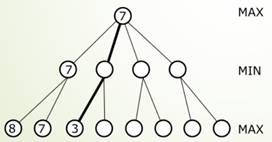
\includegraphics[width=\textwidth]{AlphaBetaPruning1.png}           
    \end{subfigure}
    ~
    \begin{subfigure}[b]{0.3\textwidth}
        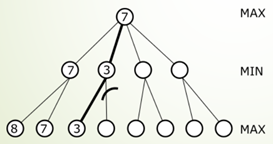
\includegraphics[width=\textwidth]{AlphaBetaPruning2.png}       
    \end{subfigure}
    \caption{An example of Alpha Beta Pruning.} % Caption beneath both of the images.
    \label{fig:AlphaBetaPruningA}
  \end{figure}

Figure \ref{fig:AlphaBetaPruningA} shows how first the leftmost branches are explored 
and the minimizer picks “7” which is stored in the variable Alpha. 
After that the second leftmost branch is explored and the Minimizer is presented with a choice that is smaller than 7.
Given that there is a choice smaller than Alpha present already, and it is the Minimizer’s turn to choose, 
meaning that it will undoubtedly have a chance to pick a value smaller than Alpha, 
it would not be worth it for the Maximizer to explore the rest of the branch and the branch is pruned as seen 
in figure \ref{fig:AlphaBetaPruningA}.

\begin{figure}[!t]
    \centering % Centering requirement met
    \begin{subfigure}[t]{0.3\textwidth}
        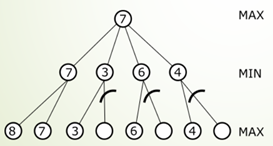
\includegraphics[width=\textwidth]{AlphaBetaPruning3.png}
    \end{subfigure}
    ~
    \begin{subfigure}[t]{0.3\textwidth}
        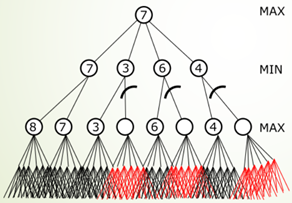
\includegraphics[width=\textwidth]{AlphaBetaPruning4.png}
    \end{subfigure}
    \caption{An example of many branches being pruned.} % Caption beneath both of the images.
    \label{fig:AlphaBetaPruningB}
  \end{figure}

Alpha Beta Pruning can potentially prune a lot of branches and 
thus make the examination of choices or moves through Minimax considerably faster 
than if it simply went through every single branch as seen in figure~\ref{fig:AlphaBetaPruningB}.

\subsection{Implementation of Alpha/Beta Pruning}
\label{subsec:Implementation of Alpha/Beta Pruning}

This section shows the changes to the minimax function and more, which was added to version 3 of the notebook in the code folder. This was done to better see the results of the pruning. 
First thing that was done was to add a counter to the minimax function in both version 3 and 4 of the code. This counter increments every time a new future move is considered. 
The idea was to show a count of how many moves the AI had considered before making the most rational choice. This way the number of considered moves on both versions of the code could be compared:
one before implementing pruning and one after.

\begin{lstlisting}[language=python, caption={python example}, label={Script}, basicstyle=\ttfamily\small]
    def minimax(board, depth, alpha, beta, isMax):
        global count 
        score = evaluate(board)
        count += 1
        if score == 10: 
            return score
        if score == -10:
            return score
        if board.count(EMPTY) == 0:
            return 0
        
        if isMax:
            maxEval = float('-inf')
            for move in all_possible_moves(board, AI):
                evaluation = minimax(move, depth + 1, alpha, beta, not isMax)
                maxEval = max(maxEval, evaluation)
                alpha = max(alpha, evaluation)
                if beta <= alpha:
                    break
            return maxEval
        else:
            minEval = float('inf')
            for move in all_possible_moves(board, HUMAN):
                evaluation = minimax(move, depth + 1, alpha, beta, not isMax)
                minEval = min(minEval, evaluation)
                beta = min(beta, evaluation)
                if beta <= alpha:
                    break
            return minEval
\end{lstlisting}

To implement Alpha Beta Pruning 2 more parameters had to be added to the function: alpha and beta. These start with the values -infinity and infinity.
The recursive call was then updated to have these arguments included. For the maximizer the alpha value was set to whichever is greater between the current alpha value and the evaluation.
Likewise it is done for the minimizer between which is lesser of beta's current value and the evaluation. This means that every time the minimax function is run, the alpha value is updated if it is the maximizing players turn. 
Likewise the beta value is updated on the minimizing players turn.
No matter whose turn it is beta is checked to see if is less than or equal to alpha, and if this is true, the rest of the moves are pruned.
\clearpage